\documentclass{article}
\usepackage{tikz}
\begin{document}

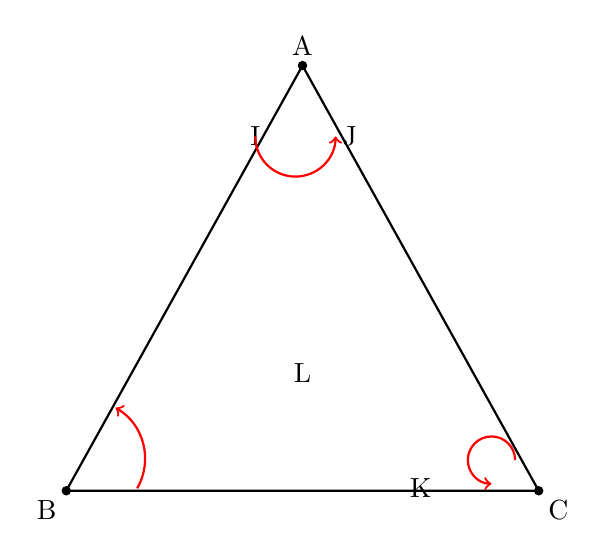
\begin{tikzpicture}[scale=3]
    % Coordonnées des sommets
    \coordinate (A) at (0,1.8);
    \coordinate (B) at (-1,0);
    \coordinate (C) at (1,0);

    % Triangle
    \draw[thick] (A) -- (B) -- (C) -- cycle;

    % Points nommés
    \fill (A) circle(0.02) node[above] {A};
    \fill (B) circle(0.02) node[below left] {B};
    \fill (C) circle(0.02) node[below right] {C};

    % Angle orienté en A (de AB vers AC)
    \node at (-0.2,1.5) {I};
    \node at (0.2,1.5) {J};
    \draw[->, thick, red] (-0.2,1.5) arc[start angle=180, end angle=360, radius=0.17];

    % Angle orienté en B (de BC vers BA → sens antihoraire donc 330 à 240)
    \draw[->, red, thick] (B)++(0.3,0.01) arc[start angle=330,end angle=420,radius=0.25];

    % Angle orienté en C (de CB vers CA → sens antihoraire donc 150 à 90)
    \node at (0.5,0.01) {K};
    \node at (0.,0.5) {L};
    \draw[->, thick, red] (0.9,0.13) arc[start angle=0, end angle=270, radius=0.1];
    %\draw[->, red, thick] (C)++(-0.3,0.01) arc[start angle=150,end angle=90,radius=0.25];
\end{tikzpicture}

\begin{tikzpicture}
    \draw[->, thick, red] (0,0) arc[start angle=0, end angle=270, radius=1];
    \node at (0,0) {D};
    \node at (-2,0) {E};
    \node at (-1,0) {O};

    
    \draw[->, thick, red] (5,0) arc[start angle=0, end angle=-90, radius=1];
    \node at (5,0) {F};
    \node at (3,0) {F};
\end{tikzpicture}

\end{document}